\documentclass[10pt]{standalone}
\usepackage{amsmath}
\usepackage{amssymb}
\usepackage[utf8]{inputenc}
\usepackage{pgf,tikz,pgfplots}
\pgfplotsset{compat=1.15}
\usetikzlibrary{arrows}
\pagestyle{empty}

\begin{document}

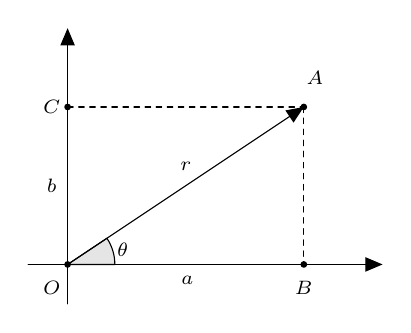
\begin{tikzpicture}[line cap=round,line join=round,>=triangle 45,x=1.0cm,y=1.0cm]
\draw[->] (-0.5,0.) -- (4.,0.);
\draw[->] (0.,-0.5) -- (0.,3.0);
\clip(-0.5,-0.5) rectangle (4.,3.);
\draw [shift={(0.,0.)},color=black,fill=black,fill opacity=0.10000000149011612] (0,0) -- (0.:0.6) arc (0.:33.69006752597979:0.6) -- cycle;
\draw [->] (0.,0.) -- (3.,2.);
\draw [dash pattern=on 2pt off 2pt] (0.,2.)-- (3.,2.);
\draw [dash pattern=on 2pt off 2pt] (3.,2.)-- (3.,0.);
\begin{scriptsize}
\draw [fill=black] (0.,0.) circle (1.0pt);
\draw[color=black] (-0.2,-0.3) node {$O$};
\draw [fill=black] (3.,2.) circle (1.0pt);
\draw[color=black] (3.14,2.37) node {$A$};
\draw[color=black] (1.5,1.25) node {$r$};
\draw[color=black] (0.7,0.19) node {$\theta$};
\draw [fill=black] (0.,2.) circle (1.0pt);
\draw[color=black] (-0.2,2.0) node {$C$};
\draw[color=black] (1.52,-0.2) node {$a$};
\draw [fill=black] (3.,0.) circle (1.0pt);
\draw[color=black] (3.0,-0.3) node {$B$};
\draw[color=black] (-0.2,1.0) node {$b$};
\end{scriptsize}

\end{tikzpicture}
\end{document}